\chapter{Theory}

\section{Definitions}


\subsection{Symmetric/Asymmetric Ciphers}

\begin{mydef}
\begin{minipage}[t]{0.8\textwidth}
    A cipher is symmetric if the encryption $E$ and the decryption $D$ use the same key $k$.
\end{minipage}
\end{mydef}

\begin{mydef}
\begin{minipage}[t]{0.8\textwidth}
    A cipher is asymmetric if the encryption $E$ and the decryption $D$ do not the same key. The encryption key is often called "public key" and the decryption one "private key".
\end{minipage}
\end{mydef}

The symmetric-key encryption is the oldest class of cryptography process. The major flaw of symmetric ciphers is the obligation for both parties (sender and receiver) to share the secret (the key). Nowadays, it is recommended to use non-symmetric encryption (also known as public-key encryption).

%\subsection{Computationally equivalence}
%Definition : two distributions $P_1$ and $P_2$ are computationally equivalent if , %for every "efficient" polynomial statistical test A, \\

%$ | Pr[A(X) == 1  - Pr[A(X) == 1] |  $ \\
%$   X <- P_1      X <- P_2              $ \\
%X chosen uniformly dans les distributions.

%\section{Probability Remainder}

\section{ Pseudo-Random Generation }

\subsection{Statistical test for Randomness}

Pseudorandomness is the property of a function to appear random, while being completely deterministic. In cryptography, the pseudorandomness property for a bit generator is an important one : the security is often built upon it since the attacker cannot predict the output. That's why a lot of different statistical test were conceived to separate true pseudorandom generators from broken ones (bit-frequency, chi-square Test, arithmetic mean, ...).

\begin{mydef}
A statistical test is an algorithm which, given a generator, output 0 or 1 based on the stream of numbers generated, 1 being random and 0 deterministic.
\end{mydef}

\paragraph{Advantage \\}
\label{sec:advantage}

Let F an oracle\footnote{an oracle is a computational black box} which we want to study and G a perfect one implementing true randomness. The advantage $Adv$ over F, using the statistical test A, is: 
\begin{mydef}
$Adv_{F} [A,G] = | Pr[A(G(k)) == 1  - Pr[A(G(r)) == 1] | \in  [0,1] $
\end{mydef}

An advantage "close to one"\footnote{it really depends on the security margin} is considered to break the pseudorandom function, because the test A can distinguish pseudo-randomness from true randomness.


\subsection{Pseudo-Random Functions   (PRF)}

A pseudo-random function is a fairly easily computable function (~polynomial) which simulate randomness while being completely deterministic.

\paragraph{Definition \\}
Let $F$ a function from $KxD$ to $R$ which maps a two set (the domain $M$ and the range $R$) using a key parameter from $K$ : the function F is a PRF if no efficient adversary with significant advantage can distinguish F from a random oracle. Pseudo-random functions are vital tools in the construction of cryptographic primitives.

\paragraph{Secure PRF \\}
\label{sec:IND-Game-PRF}

A pseudorandom function is secure if an attacker cannot solve the following game with a significant advantage :

\begin{figure}[h!]
	\centering
		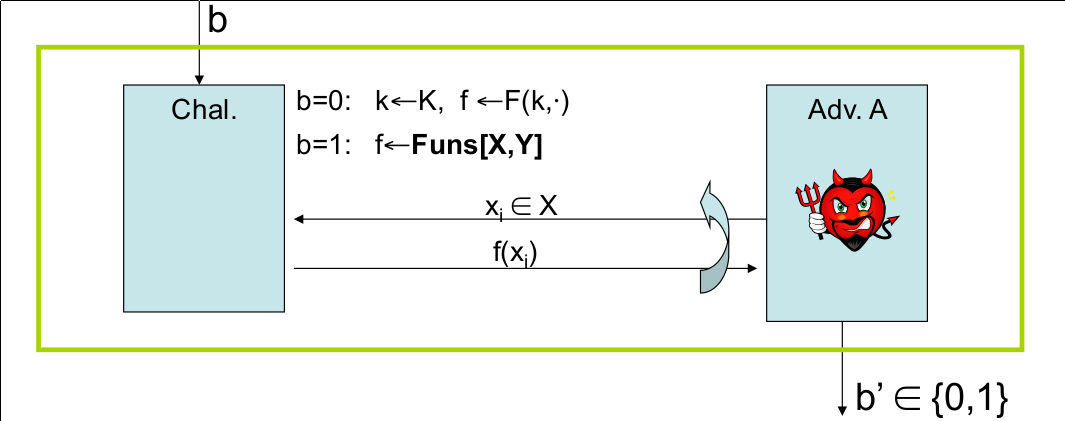
\includegraphics[width=0.7\textwidth]{secure-PRF.png}
	\caption{indistinguishability game for PRF}
	\label{fig:Cipher}
\end{figure}

Let b a binary value and $F: X\times K \rightarrow Y$  a PRF from $X$ to $Y$. If $b$ is null, the oracle will chose a random key $k\in K$, otherwise it will choose a complete random function $f:X->Y$. Then the adversary A submit one or several value(s) $x_i \in X$ and get the result $y_i \in Y$, from either the pseudo-random function or the randomly chosen one (according to the value of $b$). The attacker must find which function the oracle used, and if it find it with an advantage(see \ref{sec:advantage}), the PRF is considered insecure.


\subsection{Pseudo-Random Permutation   (PRP)}


\paragraph{Definition \\}

A PRP differs from a PRF in the way that the domain $D$ and the range $R$ are the same. Since the function map the two same sets, we can deduce that $E(k,.)$ ( k is fixed) is bijective : it is a permutation then.
A major propriety of the PRP (comparatively to the PRF) is that the PRP can be inverted, thus improving the decoding speed.\footnote{Another useful property is that permutation can be chained or cascaded since they all have the same working domain.}

\paragraph{Secure PRP \\}


\begin{figure}[ht!]
	\centering
		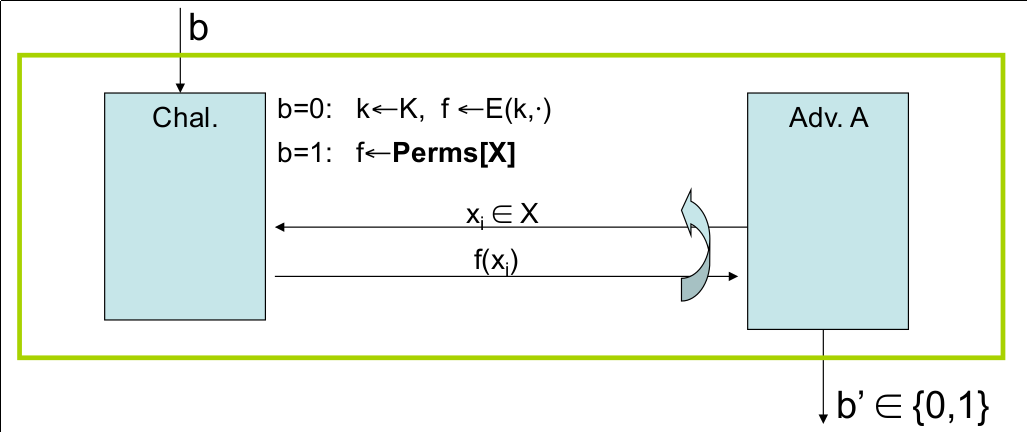
\includegraphics[width=0.7\textwidth]{secure-PRP.png}
	\caption{indistinguishability game for PRP}
	\label{fig:Cipher}
\end{figure}

The challenge for PRP is not much different from the one on PRF : see \ref{sec:IND-Game-PRF}.

\subsection{Pseudo Random Generator     (PRG)} 


\paragraph{Definition \\}

A pseudo random generator (PRG) is a deterministic bit generator with the property of  unpredictability :
\begin{mydef}
$ G : \llbracket  0,1 \rrbracket ^s -> \llbracket  0,1 \rrbracket ^n $  with  $n>>s$. 

$ G : \flushright	 $S = \llbracket  0,1 \rrbracket ^s$ is often called "the seed" and is randomly chosen. 

\end{mydef}

Stream ciphers are easily built from PRG : $c = m \oplus G(k) $  (one time pad with pseudo-random generator )


\paragraph{Secure PRG \\}
A PRG is secure if, for all "efficient" statistical test A, $Adv(A,G)$ is negligible.

On a side note, we don't know all the existing efficient statistical tests so we can't prove that PRG is secure, we can only prove we didn't found an efficient test which break it.


\section{Confidentiality}
\subsection{Perfect Secrecy}

\begin{mytheorem}[Shannon perfect secrecy]
    $\forall m_1,m_2$ such as $len(m_1) = len(m_2)$, 
    $Pr[E(k,m_1) = c] = Pr[E(k,m_2) = c]$  \flushright (k uniform in K)
\end{mytheorem}

In layman terms, perfect secrecy means that, given two messages and the ciphertext of one of the two plaintext messages, the attacker cannot know from which message the ciphertext has been created (equal probability). A corollary is, under perfect secrecy conditions, the key space $K$ cardinality must be equal or larger than the ciphertext space $C$ cardinality, which has to be equal or larger than the message space $M$ cardinality :
\begin{mytheorem}[Shannon perfect secrecy corollary]
    $ |M| \leq |C| \leq |K| $. 
\end{mytheorem}


\subsection{Semantic Security}

The semantic security is a weaker form of Shannon's perfect secrecy (which is not usable in reality) : the distributions $P_1 = Pr[E(k,m_1) = c , k<- K]$ and $P_2$ does not have to be equal, just computationally equivalent.

\paragraph{Challenge}
The semantic security is often defined using a "challenge" : an experiment of though where and adversary has to find an important information given a certain protocol and certain rights. The challenge is the following one :

\begin{figure}[ht!]
	\centering
		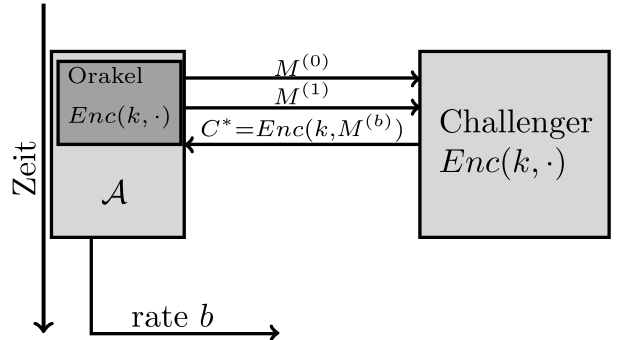
\includegraphics[width=0.7\textwidth]{IND-CPA-Game.png}
	\caption{Semantic security challenge}
	\label{fig:SemanticSecurityChallenge}
\end{figure}

The challenger (the "defender") choose a fixed-key and a variable $b$ randomly from two values ( 0 and 1 to be simple). The attacker then will send the challenger $2*n$ messages (plain or encrypted) and the challenger only process half of them (given the value b) and send the result back to the attacker.\\
The attacker has to estimate the value $b$ chosen : if the attacker can guess the value of b with a significant advantage, the encryption cipher is considered insecure. Otherwise, it has semantic security against the corresponding attack channel.

\paragraph{Semantic Security against Chosen Plaintext Attack (CPA)\\}

In this configuration, the attacker can choose which plaintext message(s) to send to the challenger, and has the result of the encryption of half of them. 

\begin{mytheorem}[Semantic Security under CPA]
$E$ is semantically secure  under chosen plaintext attack if, for all adversary A,
     
\flushright	 for all adversary A, $Adv_{CPA}[A,E] = Pr()$ is negligible.
\end{mytheorem}

\paragraph{Semantic Security against Chosen Ciphertext (Adaptive) Attack ($CCA-1$/$CCA-2$)\\}

In this configuration, the attacker can choose which ciphertext message(s) to send to the challenger, and has the result of the decryption of half of them. Under $CCA-2$ he can also makes incremental changes to the ciphertext sent given the output the previous decryption, enabling linear and differential attacks. \\
The $CCA$ assumption allow the attacker a wide range of access to information : the protocols which are secure against $CCA$ are extremely useful since they can withstand a great variety of attacks \footnote{of course, there still are side-channel attacks.}.

\section{Integrity}

\subsection{Secure MAC}

The challenge used to define MAC security is a bit different from the one for semantic security : the challenger choose a key randomly. The attacker can submit $n$ messages $m_i$ and receive their corresponding tags $t_i$. Then he can submit \underline{a new} forged message-tag pair $(m,t)$ which will be verified by the challenger. If the challenger certified the pair to be true, the MAC protocol is considered insecure, otherwise it is secure.

\begin{figure}[ht!]
	\centering
		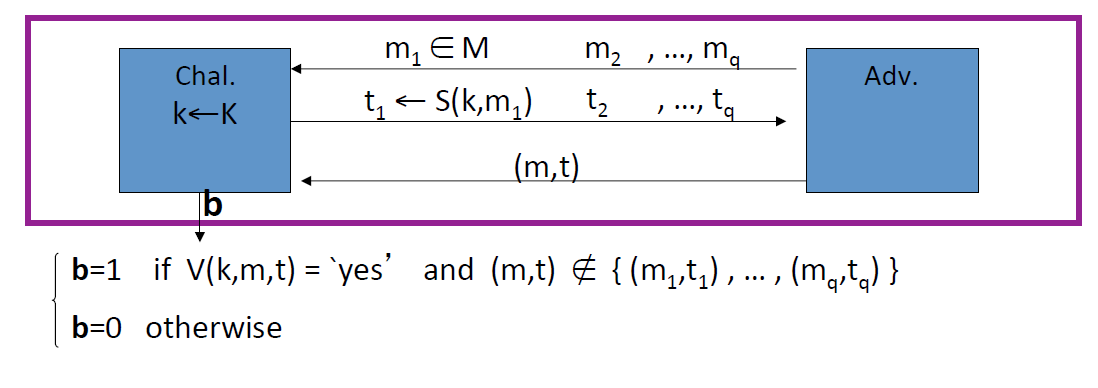
\includegraphics[width=0.7\textwidth]{IND-CPA-MAC-Game.png}
	\caption{MAC integrity challenge}
	\label{fig:MACIntegrityChallenge}
\end{figure}

\begin{mydef}
I$=(S,V)$ is considered secure if $\forall$ efficient statistical test A, 
\begin{flushright}
$Adv_{MAC}[A,I] = Pr[ b == 1] $ is negligible.
\end{flushright} 
\end{mydef}


%\section{Number Theory}
